%\chapter{Experimental method} 

\section{$^3$He($K^-,n$) reaction at 1 GeV/$c$}
To search for the $K^-pp$ state, we adopted the $^3$He($K^-,n$) reaction at 1 GeV/$c$. The formation spectrum is derived by means of the missing mass spectroscopy of the incoming kaon and the outgoing neutrons. In the current experiment, we focus on neutrons at very forward angle. The neutron missing mass $M_X$ can be expressed as,
\begin{eqnarray}
M_X = \sqrt{(M_{^3\rm{He}}+\sqrt{M_{K^-}^2+\bf{p}_{K^-}^2}-\sqrt{M_{n}^2+\bf{p}_n^2})^2-(\bf{p}_{K^-}-\bf{p}_n)^2},
\end{eqnarray}
where $M_{^3\rm{He}}$, $M_{K^-}$, and $M_n$ are masses of a $^3$He, a negative kaon beam and a neutron, and $\bf{p}_{K^-}$ and $\bf{p}_n$ are three momenta of the kaon beam and neutron, respectively.

We used kaon beam at the K1.8BR beam-line in the Hadron experimental facility at J-PARC, which is explained in Sec. 2.3 and Sec. 2.4. The description about the beam line detectors measuring ${\bf p_{K^-}}$ is given in Sec. 2.6. As the experimental target, we developed a liquid $^3$He cryogenic target as appears in Sec 2.7. Momenta of the forward neutrons (${\bf p_n}$) were measured by time-of-flight (TOF) method together with particle identification by using charge veto technique. These systems are described in Sec. 2.9. Note that a typical momentum of a forward-going neutron emitted from the $K^-pp$ formation is 1.2$\sim$1.4 GeV/$c$. In addition, we installed decay-particle detectors that surround the $^3$He target to determine the reaction vertex point. Section 2.8 is dedicated for a cylindrical detector system developed for this purpose. Finally, we describe the trigger scheme and a data acquisition system in Sec. 2.10.
\section{Experimental requirement}
Before describing the detailed experimental setup, the experimental requirements are discussed in terms of the experimental resolution.

The experimental resolution, namely, the missing mass resolution, is important not only for the search for a discrete peak but also the precise determination of the natural width of the state. Since the expected binding energy and the width of $\bar KNN$ systems are in the order of 10 MeV, the missing mass resolution is required to be $\sim$10 MeV/$c^2$ in the region of interest. Considering that order of $10^{-3}$ resolution of the kaon beam momentum is easily achievable with a conventional magnetic spectrometer, the main contribution of the missing mass resolution comes from the forward neutron momentum measurement. A calculated momentum and missing mass resolutions in a very simple case are shown in Fig.~\ref{fig-calcres}. Here we assumed the flight length is 15 m for a forward neutron measurement and the kaon beam momentum is 1 GeV/$c$. To achieve the required resolution, we need time-of-flight resolution better than 200 ps including uncertainties of the reaction vertex in the target and the neutron detection point. 

  \begin{figure}[]
   \begin{center}
    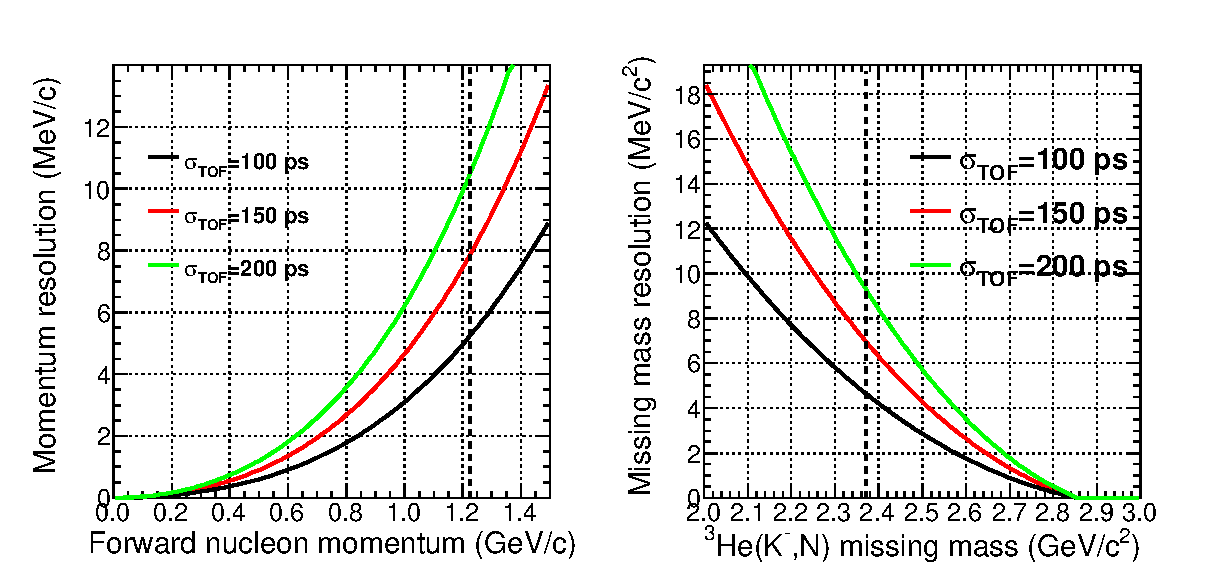
\includegraphics[width=\columnwidth]{fig/calcres.eps}
    \caption{Simple calculation of resolutions of the forward nucleon momentum and missing mass. }
    \label{fig-calcres}
   \end{center}
  \end{figure}  
